\usepackage{xcolor}
\usepackage{afterpage}
\usepackage{pifont,mdframed}
\usepackage[bottom]{footmisc}
\usepackage{minted}

\createsection{\Grader}{Grader di prova}
\newcommand{\inputfile}{\texttt{stdin}}
\newcommand{\outputfile}{\texttt{stdout}}
\makeatletter
\renewcommand{\this@inputfilename}{\texttt{stdin}}
\renewcommand{\this@outputfilename}{\texttt{stdout}}
\renewcommand{\this@syllabuslevel}{5}
\renewcommand{\this@custdifficulty}{3}
\makeatother

% % % % % % % % % % % % % % % % % % % % % % % % % % % % % % % % % % % % % % % % % % %
% % % % % % % % % % % % % % % % % % % % % % % % % % % % % % % % % % % % % % % % % % %
Marco si sta annoiando perché il gioco \textit{Squaremania} gli risulta troppo semplice.
Per fortuna viene a sapere che esiste una nuova versione del gioco: \textit{Squaremania 2}.
\begin{figure}[h]
    \centering
    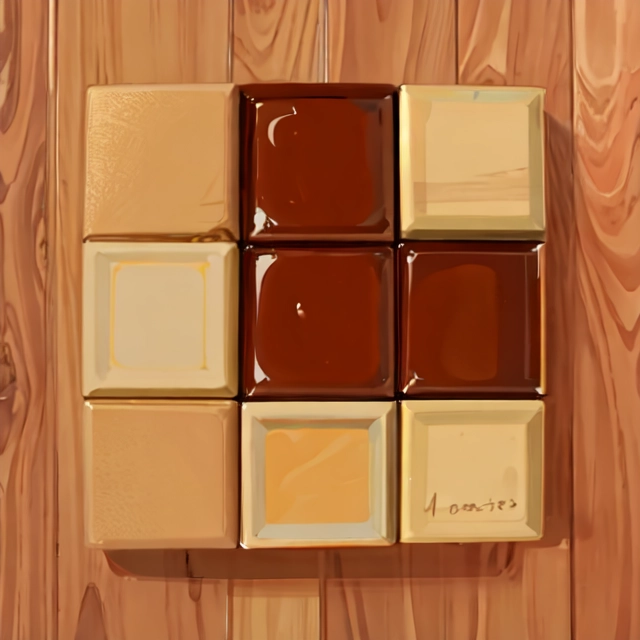
\includegraphics[width=0.4\textwidth]{./woodoku2.png}
    \caption{L'icona di \textit{Squaremania 2}.}
\end{figure}

Il gioco è simile: vengono forniti al giocatore $N$ cubetti di legno $1\times1$, ma a differenza della
versione precedente non è obbligatorio formare un solo quadrato. L'obiettivo di \textit{Squaremania 2}
è quello di raggruppare i cubetti nel minor numero di quadrati possibile.

Ad esempio, se venissero forniti $13$ cubetti, si potrebbe formare un quadrato $3\times3$ e uno $2\times2$,
e si può dimostrare che non esiste soluzione migliore.

Aiuta Marco trovando una soluzione ottimale al problema.
\begin{warning}
    Possono esistere più soluzioni ottimali. In tal caso, qualsiasi delle soluzioni ottimali verrà considerata corretta.
\end{warning}


\Implementation

Dovrai sottoporre un unico file, con estensione \texttt{.cpp}.

\begin{warning}
    Tra gli allegati a questo task troverai un template \texttt{squaremania2.cpp} con un esempio di implementazione.
\end{warning}

Il file di input è composto da $1$ riga:
\begin{itemize}
    \item Riga 1: l'intero $N$.
\end{itemize}

Il file di output è composto da $1$ riga:
\begin{itemize}
    \item Riga 1: Il numero di quadrati.
    \item Riga 2: Le lunghezze dei lati dei quadrati, separate da uno spazio.
\end{itemize}

% % % % % % % % % % % % % % % % % % % % % % % % % % % % % % % % % % % % % % % % % % %
% % % % % % % % % % % % % % % % % % % % % % % % % % % % % % % % % % % % % % % % % % %

\Constraints

\begin{itemize}[nolistsep, itemsep=2mm]
    \item $1 \le N \le 15\:000$.
\end{itemize}

% % % % % % % % % % % % % % % % % % % % % % % % % % % % % % % % % % % % % % % % % % %
% % % % % % % % % % % % % % % % % % % % % % % % % % % % % % % % % % % % % % % % % % %

\Scoring

Il tuo programma verrà testato su diversi test case raggruppati in subtask.
Per ottenere il punteggio relativo ad un subtask,
è necessario risolvere correttamente tutti i test che lo compongono.

\IIOTsubtask{0}{1}{Casi d'esempio.}

\IIOTsubtask{50}{1}{$N \le 11$}

\IIOTsubtask{50}{3}{Nessuna limitazione aggiuntiva.}


% % % % % % % % % % % % % % % % % % % % % % % % % % % % % % % % % % % % % % % % % % %
% % % % % % % % % % % % % % % % % % % % % % % % % % % % % % % % % % % % % % % % % % %

\Examples

\begin{example}
    \exmpfile{squaremania2.input0.txt}{squaremania2.output0.txt}%
    \exmpfile{squaremania2.input1.txt}{squaremania2.output1.txt}%
    \exmpfile{squaremania2.input2.txt}{squaremania2.output2.txt}%
\end{example}

% % % % % % % % % % % % % % % % % % % % % % % % % % % % % % % % % % % % % % % % % % %
% % % % % % % % % % % % % % % % % % % % % % % % % % % % % % % % % % % % % % % % % % %

\Explanation

Il primo caso d'esempio è quello descritto nel testo del problema.

Nel secondo caso d'esempio, si possono formare $3$ quadrati di dimensioni $1\times1$ e uno di dimensione $2\times2$.

Nel terzo caso d'esempio conviene formare un quadrato $50\times50$ e uno $17\times17$.